\subsubsection{Les risques politiques.}
%Comment les fakes news peuvent aider à cacher des scandales politiques.
L'institutionnalisation des Fake News est l'un des plus gros risques politiques.
En effet rien de pire qu'une Fake News qui a pour pseudo-autorité un état.
Un état niant les faits devient répressifs.
%Exemple les alternatives facts de l'institution de Donald Trump.
\begin{center}
 \begin{figure}[h]
  \begin{subfigure}{.5\textwidth}
   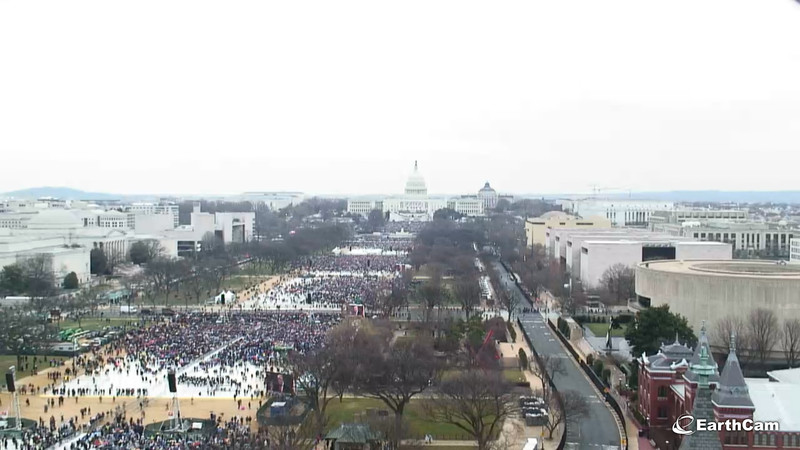
\includegraphics[scale=0.240]{../../img/trumpvswomen/trump.png}
   \caption{L'inauguration de Trump}
   \label{fig:sub1}
  \end{subfigure}
  \begin{subfigure}{.5\textwidth}
   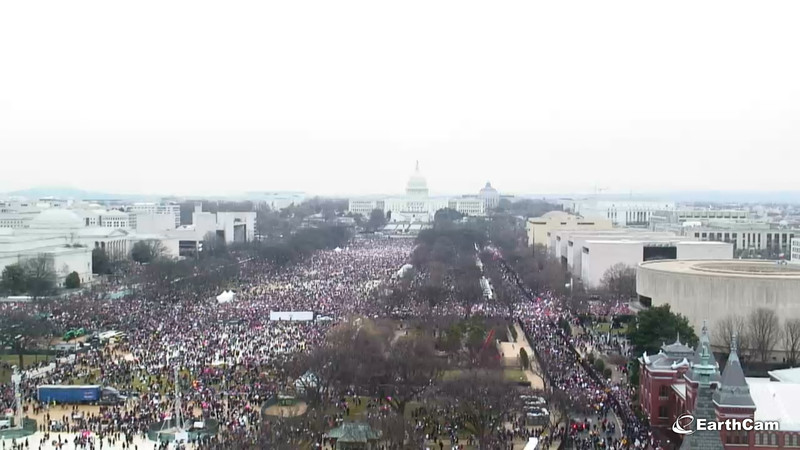
\includegraphics[scale=0.240]{../../img/trumpvswomen/women.png}
   \caption{Women’s March}
   \label{fig:sub2}
  \end{subfigure}
  \caption{Deux photos d'événements du National Mall à Washington}
  \label{fig:test}
 \end{figure}
\end{center}

L'inauguration de Trump et la Women's March avaient fait beaucoup de bruit.
Les partisans pro-Trump seraient soi-disant en plus grand nombre que les partisans de la Women's March.
Nous pourrions croire la version officielle.
Mais apparemment sans comptage, il y avait plus de participants à la Women's March.
L'État américain avaient tenté de faire passer cela pour des faits alternatifs.
Ce qui n'a pas beaucoup de sens.
Certes, nous observons tous le réel de manière différente, mais ce n'est pas une raison pour faire du relativisme et conclure à des faits alternatifs.
De plus comment définir des faits alternatifs ?
Prendre des faits et les dénaturer à des fins idéologiques ne nous donne pas raison sur la réalité.
En somme, les Fake News peuvent servir à cacher des scandales politiques.

D'autres Fake News institutionnalisées peuvent servir à des particuliers pour qu'ils puissent s'enrichir, ou à ne pas payer d'amende.
Par exemple, nier le réchauffement climatique est très pratique quand on est l'un des pays les plus polluant au monde.
\subsubsection{Les risques sanitaires.}
%Comment la santé peut être mise en danger par de fausse informations?
Beaucoup de Fake News portent sur les domaines sanitaires.
Comme nous l'avons vu précédemment avec les vaccins, les Fake News développent une méfiance pour la médecine conventionnelle.
Pour reprendre l'exemple des vaccins, il faut savoir que des cas de rougeole mortels sont réapparus ces dernières années. \textcolor{red}{(sources ?)}
Ne pas se vacciner entraîne un baisse de la couverture vaccinale.
Le rapport bénéfice/risque est plus que positif pour la vaccination.
Aucun des effets indésirables notoires suspectés n'a trouvé un protocole testable positif.
Nous n'avons que des affirmations pseudo-scientifiques et des hypothèses contre.
En somme, la désinformation, autour de la médecine notamment, peut couter la vie.

\subsubsection{Détournement des news vers des sujets clivants.}
Les Fake News peuvent être colportées par des personnes convaincues de leur véracité.
Le but ultime d'une Fake News est d'être considéré comme une vraie information.
Les Fake News détournent l'attention de la population vers des problèmes factices et souvent résolus depuis des années. En somme les Fake News sont une perte de temps. Elles nous empêchent de nous focaliser sur de vrais problèmes ; car l'on doit démystifier des faits irréels.
